\documentclass[xcolor=pdftex,dvipsnames,table,mathserif]{beamer}
%\usepackage{subfigure}
\usepackage{amsbsy}
\usepackage{tikz}
\usetikzlibrary{arrows}
\usepackage{amsmath,graphicx,dsfont,color}
\usepackage{amsfonts}
\usepackage{amssymb}
\usepackage{array}

\usepackage{subfig}

% makes the subfig package work
\makeatletter
\let\@@magyar@captionfix\relax
\makeatother

% subfigure counter resets every frame
\makeatletter
\@addtoreset{subfigure}{framenumber}
\makeatother

% First author and year
\bibliographystyle{apalike}

% This sets the list items of the bibliography to the same symbol used for citation.
\setbeamertemplate{bibliography item}{\insertbiblabel}

% This avoids extralines for different entries
\setbeamertemplate{bibliography entry title}{}
\setbeamertemplate{bibliography entry location}{}
\setbeamertemplate{bibliography entry note}{}

\DeclareMathOperator*{\argmin}{arg\,min}
\DeclareMathOperator*{\argmax}{arg\,max}
%Definitiona

\newcommand{\x}{\mathbf{x}}
\newcommand{\X}{\mathbf{X}}
\newcommand{\W}{\mathbf{W}} %Weight
\newcommand{\bais}{\mathbf{b}}%Bais
\newcommand{\act}{\texttt{g}}%Activation
\newcommand{\loss}{L}
\newcommand{\pdata}{\hat{p}_{\texttt{data}}}
\newcommand{\nsize}{N}
\newcommand{\nfeatures}{P}
\newcommand{\param}{\boldsymbol{\theta}}
\newcommand{\featmap}{\boldsymbol{\phi}}
\newcommand{\EV}{\mathbb{E}}







\usepackage{physics}

\graphicspath{{../graphics/}}

\AtBeginSection[]{
  \begin{frame}{Contents}
    \tableofcontents[currentsection, hideothersubsections]
  \end{frame}
}

\AtBeginSubsection[]{
  \begin{frame}{Contents}
    \tableofcontents[currentsection, subsectionstyle=show/shaded/hide]
  \end{frame}
}

\setbeamertemplate{footline}[frame number]{}
\setbeamertemplate{navigation symbols}{}
\setbeamertemplate{section in toc}[square]
\setbeamertemplate{items}[square]

%% For image credits on image bottom right
\usepackage[absolute,overlay]{textpos}
\setbeamercolor{framesource}{fg=gray}
\setbeamerfont{framesource}{size=\tiny}
\newcommand{\source}[1]{\begin{textblock*}{4cm}(8.7cm,8.6cm)
    \begin{beamercolorbox}[ht=0.5cm,right]{framesource}
        \usebeamerfont{framesource}\usebeamercolor[fg]{framesource} Credits: {#1}
    \end{beamercolorbox}
\end{textblock*}}


\title{Deep learning in practice}
\author{E. Decencière}
\date{MINES ParisTech\\
  PSL Research University\\
  Center for Mathematical Morphology
}
\titlegraphic{
\includegraphics[height=1.7cm]{../graphics/logoemp}}

\useinnertheme{rounded}
\usecolortheme{rose}

%%%%%%%%%%%%%%%%%%%%%%%%%%%%%%%%%%%%%%%%%%%%%%%%%%%%%%%
%%%%%%%%%%%%%%%%%%%%%%%%%%%%%%%%%%%%%%%%%%%%%%%%%%%%%%%
\begin{document}

\frame{\titlepage}

\frame{
  \frametitle{Contents}
  \tableofcontents[hidesubsections]
}

%%%%%%%%%%%%%%%%%%%%%%%%%%%%%%%%%%%%%%%%%%%%%%%%%%
%%%%%%%%%%%%%%%%%%%%%%%%%%%%%%%%%%%%%%%%%%%%%%%%%%
\section{Introduction}


%%%%%%%%%%%%%%%%%%%%%%%%%%%%%%%%%%%%
\begin{frame}{}
\centering
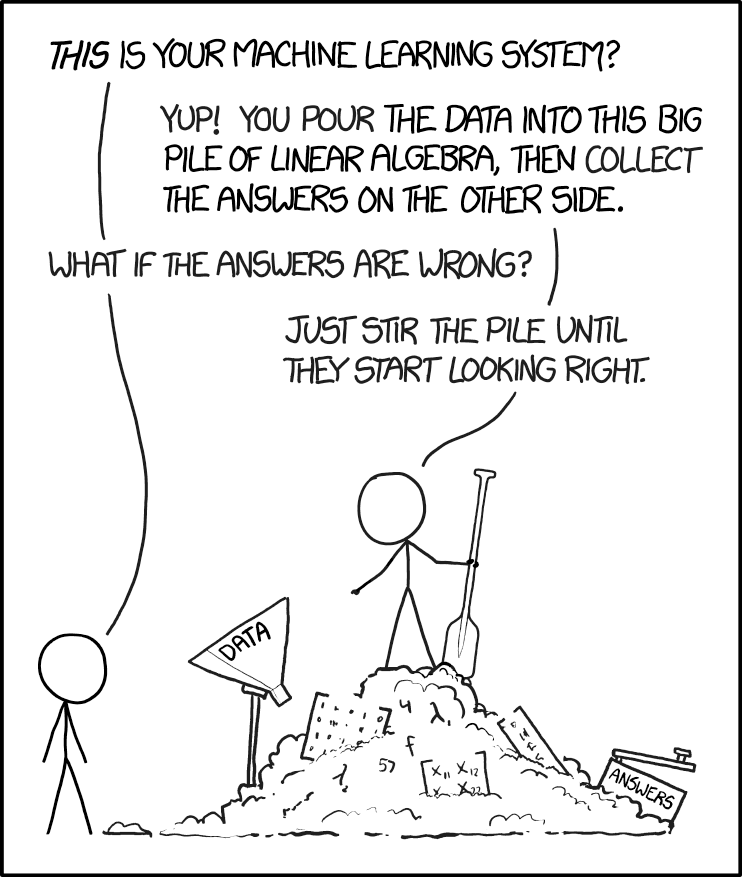
\includegraphics[height=\textheight]{xkcd_machine_learning}
\source{xkcd.com\\ (CC BY-NC 2.5)}
\end{frame}

%%%%%%%%%%%%%%%%%%%%%%%%%%%%%%%%%%%%
\begin{frame}{Practicing deep learning}

  In every discipline theory and practice are important. In deep learning, practice is essential.

  \begin{itemize}[<+->]
  \item We lack theoretical understanding of the success of deep learning
  \item Many common techniques have been adopted for empirical reasons
  \item In order to improve your skills, you have to practice a lot and read the reports by other practitioners
  \end{itemize}

  \pause

  \begin{alertblock}{}
    This state of affairs can of course be a problem in domains where security and interpretability are important, such as clinical applications.
  \end{alertblock}

\end{frame}


%%%%%%%%%%%%%%%%%%%%%%%%%%%%%%%%%%%%%%%%%%%%%%%%%%%%%
\frame{
  \frametitle{General workflow}

  \begin {itemize}[<+->]
  \item Familiarize yourself with the problem and the data
  \item Build your data set
  \item Cast the task at hand into a machine learning problem
  \item Build an architecture and train it (begin with simple ones!) or choose a pre-trained model and use transfer learning

\begin{itemize}[<+->]
  \item Analyze the results on the validation data (\alert{look} at the images!)
  \item Beware of over-fitting! Envision regularization methods.
  \item Use data augmentation. If correctly used, it cannot hurt and will probably improve the generalization power of your network.
  \item Do you need preprocessing? Post-processing?
  \item Iterate, while precisely logging all your experiments.
\end{itemize}

  \item Only at the end: test!
  \end{itemize}
}



%%%%%%%%%%%%%%%%%%%%%%%%%%%%%%%%%%%%%%%%%%%%%%%%%%
\section{Problem representation}

%%%%%%%%%%%%%%%%%%%%%%%%%%%%%%%%%%%%%%%%%%%%%%%%%%%%%
\frame{
  \frametitle{Representing your problem}

  Cast your problem into a convenient representation.

    \begin {itemize}[<+->]
    \item Understand the problem definition - discuss with the end-user
    \item Familiarize yourself with the data (input and output)
    \item Choose the right representation for your images.
    \item Define an evaluation procedure
    \end{itemize}


}


%%%%%%%%%%%%%%%%%%%%%%%%%%%%%%%%%%%%
\begin{frame}{Example: eye fundus image quality}

\begin{columns}
  \begin{column}{.4\textwidth}
    \begin{figure}[ht]
      \centering
      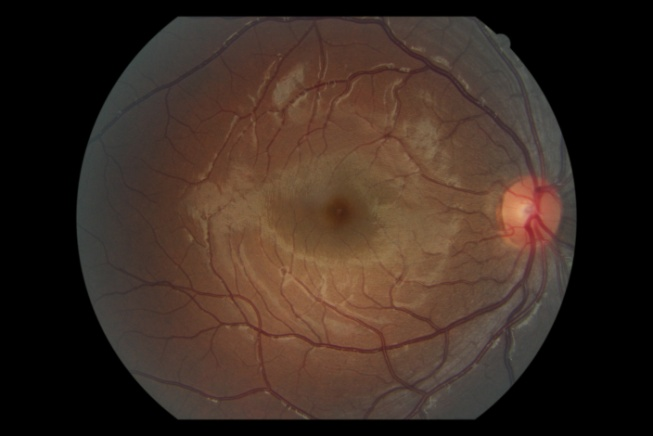
\includegraphics[width=\textwidth]{fundus1}\\
      Good quality\vspace{1em}\\
      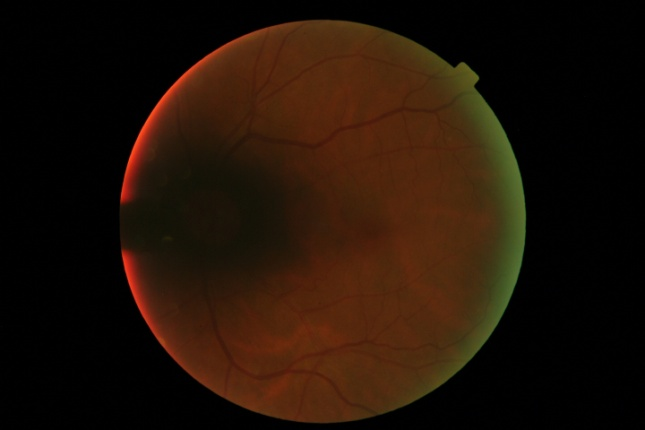
\includegraphics[width=\textwidth]{fundus2}\\
      Low quality
    \end{figure}

  \end{column}

  \begin{column}{.6\textwidth}
    \begin{block}{Problem definition}
    Quality criterion defined by the end-user: are the macula and peripheral vessels visible?
    \end{block}
    \pause
    \begin{itemize}
    \item First solution: classification (is the macula visible?)
    \item Second solution: macula segmentation
      \end{itemize}
  \end{column}
\end{columns}

\source{images from OPHDIAT database}
\end{frame}

%%%%%%%%%%%%%%%%%%%%%%%%%%%%%%%%%%%%%%%%%%%%%%%%%%
\frame{
  \frametitle{Counting cells}

    \begin{figure}
      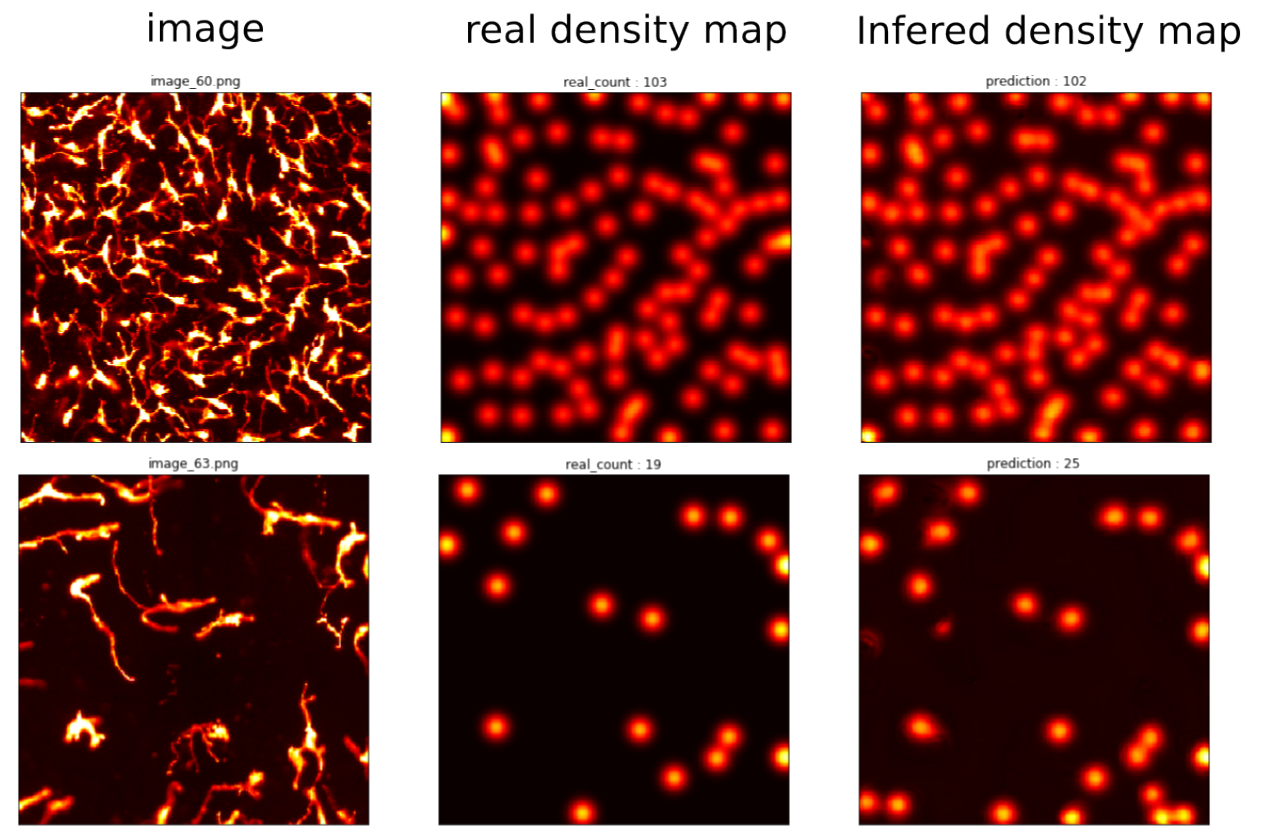
\includegraphics[width=\textwidth]{lazard}
      \source{Tristan Lazard, master thesis. In collaboration with L'Oréal.}
    \end{figure}

}


%%%%%%%%%%%%%%%%%%%%%%%%%%%%%%%%%%%%
\begin{frame}{Performance evaluation}

  \begin{itemize}
  \item Choose the right metrics and try to use a loss function that is as close as possible to these metrics
  \item Define an objective
  \end{itemize}

\end{frame}


%%%%%%%%%%%%%%%%%%%%%%%%%%%%%%%%%%%%%%%%%%%%%%%%%%%%%
\section{Data preparation}

%%%%%%%%%%%%%%%%%%%%%%%%%%%%%%%%%%%%
\begin{frame}{Building the data sets}
  \begin{itemize}
  \item Gather your images in order to build a data set that conveniently represents your problem
  \item How many images do you need?
  \item Build a proper ground-truth
  \end{itemize}

  \pause

  \begin{alertblock}{Is database constitution the main step?}
    \begin{itemize}
    \item In practical, real-world applications, this is becoming the most time-consuming step
    \item If the data set does not conveniently represent your problem you will run into difficulties
    \end{itemize}

  \end{alertblock}

\end{frame}

%%%%%%%%%%%%%%%%%%%%%%%%%%%%%%%%%%%%
\begin{frame}{Anecdote: tank detection}

  In the first years of artificial neural networks, a perceptron was trained to detect images containing tanks. Its results were quite good...
  \vspace{1em}

  \pause

  ... but in fact images containing tanks were acquired during sunny days, while images without tanks were shot with overcast weather. The network was simply detecting lighter images!
  \vspace{1em}

  \pause

  This anecdote might be a urban legend, but nevertheless is a good illustration of the problems one might run into during database preparation. More information available from:

  \centering
  \url{https://www.gwern.net/Tanks}
\end{frame}

%%%%%%%%%%%%%%%%%%%%%%%%%%%%%%%%%%%%%%%%%%%%%%%%%%%%%
\frame{
  \frametitle{What quality is needed for the ground-truth?}

  \begin{itemize}
  \item Deep learning models tend to be robust with respect to ground-truth errors
  \item In the case of segmentation, you do not need a pixel-precision high quality segmentation \cite{heller_imperfect_2018}
  \end{itemize}

}

%%%%%%%%%%%%%%%%%%%%%%%%%%%%%%%%%%%%%%%%%%%%%%%%%%%%%
\frame{
  \frametitle{Preprocessing}

  \begin {itemize}
  \item Standard statistical preprocessing: not always useful, and sometimes problematic, when applied to images. It is often enough to divide by $255$!
  \item Use other preprocessing only if really necessary.
  \end{itemize}

}


%%%%%%%%%%%%%%%%%%%%%%%%%%%%%%%%%%%%%%%%%%%%%%%%%%%%%
\frame{
  \frametitle{Data augmentation}

  \begin {itemize}
  \item Geometrical transformations: similarities
  \item Elastic transformations
  \item Noise
  \item Grey level or colour modifications
  \item Specific methods: articulated objects, \ldots
  \end{itemize}
}


%%%%%%%%%%%%%%%%%%%%%%%%%%%%%%%%%%%%
\begin{frame}{Example: plankton classification}

Plankton classification: hundred classes - a few dozen examples per class.
\vspace{2em}
\begin{columns}
  \begin{column}{.5\textwidth}
    Data augmentation:
    \begin{itemize}
    \item Geometric transformations
    \item Detect joints and simulate their functioning
    \end{itemize}
  \end{column}

  \begin{column}{.5\textwidth}
  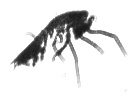
\includegraphics[width=0.4\textwidth]{kaggle_amphipod}
  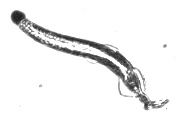
\includegraphics[width=0.4\textwidth]{kaggle_chaetognath}
  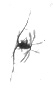
\includegraphics[width=0.2\textwidth]{kaggle_copepod}
  \end{column}
\end{columns}



\source{Kaggle plankton classification challenge (https://www.kaggle.com)}

\end{frame}

%%%%%%%%%%%%%%%%%%%%%%%%%%%%%%%%%%%%
\begin{frame}{Using simulated data}

  \begin{itemize}[<+->]
  \item Using simulated data is convenient...
  \item ... but it has to be as similar as possible to the real data
  \item A transfer learning method with real data will probably be necessary
  \item Your test data should be real
  \end{itemize}

\end{frame}


%%%%%%%%%%%%%%%%%%%%%%%%%%%%%%%%%%%%%%%%%%%%%%%%%%%%%
\section{Architecture choice and training}

%%%%%%%%%%%%%%%%%%%%%%%%%%%%%%%%%%%%
\begin{frame}{Architecture choice}

  \begin{itemize}[<+->]
  \item Begin with a standard architecture
    \begin{itemize}
    \item Classification problem: VGG, GoogLeNet, ResNet...
    \item Semantic segmentation or image transformation problem: U-Net
    \item Instance segmentation: Mask R CNN
    \end{itemize}
  \item If you are dealing with a complex problem, start with pre-learned weights and use transfer learning to adapt them to your application
  \end{itemize}

  \pause

  It is interesting to note that the rate of publication of new architectures tends to decrease.

\end{frame}


%%%%%%%%%%%%%%%%%%%%%%%%%%%%%%%%%%%%%%%%%%%%%%%%%%%%%
% \section{Training}

%%%%%%%%%%%%%%%%%%%%%%%%%%%%%%%%%%%%
\begin{frame}{Optimizing your model}

  \begin{itemize}
  \item Choose an optimizer
  \item Use regularization ($L_1$, $L_2$, dropout, noise layer ...)
  \item Add batch normalization if convergence is difficult

  \end{itemize}

\end{frame}


%%%%%%%%%%%%%%%%%%%%%%%%%%%%%%%%%%%%
\begin{frame}{Hyperparameters tuning}

  \begin{itemize}
  \item Manual tuning: might work if the number of parameter is small and the experience of the developer/researcher high
  \item Automatic tuning:
    \begin{itemize}
    \item Grid search
    \item Random search
    \item Population based approaches
    \item Etc.
    \end{itemize}
  \end{itemize}

  When working with keras, you can use keras-tuner.

\end{frame}

%%%%%%%%%%%%%%%%%%%%%%%%%%%%%%%%%%%%
\begin{frame}{Computing power}

  DL became feasible in practice thanks to the use of Graphical Processing Units (GPU). Beyond theoretical research on the subject, to work with DL you need specific hardware:
  \begin{itemize}
  \item CPUs: with many of them, and using libraries that allow parallelization, this could be a solution - in practice, it is seldom done.
  \item GPUs: this is the most common solution adopted for deep learning.
  \item TPU: Tensor Processing Units are integrated circuits specifically developed by Google for deep learning.
  \end{itemize}

\end{frame}

%%%%%%%%%%%%%%%%%%%%%%%%%%%%%%%%%%%%
\begin{frame}{Computing power}

  \begin{alertblock}{}
    \begin{itemize}
    \item   DL research and development is extremely computationally time-consuming.
    \item   However, running predictions with an already optimized model is much faster
    \end{itemize}
  \end{alertblock}
\end{frame}


%%%%%%%%%%%%%%%%%%%%%%%%%%%%%%%%%%%%%%%%%%%%%%%%%%
\section{Transfer learning}

%%%%%%%%%%%%%%%%%%%%%%%%%%%%%%%%%%%%
\begin{frame}{Problem formulation}

  In computer vision:
\begin{itemize}
\item Databases can be huge, requiring substantial computing power and making learning complex
\item In many practical applications the learning data base can be small
\end{itemize}

Transfer learning brings a solution to these problems.

\end{frame}


%%%%%%%%%%%%%%%%%%%%%%%%%%%%%%%%%%%%
\begin{frame}{Definitions \cite{pan_survey_2010}}

\begin{block}{Domain and task}

\begin{itemize}
\item A domain $D$ is a probability space ($X$, $P$), where $X$ is finite.

\item Given a domain $D = (X, P)$, a task $T$ consists
of two components: a label space $\mathcal{Y}$ and a
function $f: X \rightarrow \mathcal{Y}$, that is only known on a training set
$\{(x_i, y_i), 1 \leq i \leq n, x_i \in X,  y_i \in Y\}$.

\end{itemize}

\end{block}

\pause

\begin{block}{Transfer learning}

  Let us consider

  \begin{itemize}
  \item a \emph{source} domain $D_S$ and a task $T_S$ on that domain, and
  \item a \emph{target} domain $D_T$ and a task $T_T$ on that domain.
  \end{itemize}

Transfer learning from $(D_S, T_s)$ to $(D_T, T_T)$, where $D_S \neq D_T$ or $T_S \neq T_T$,  consists in using the knowledge in $(D_S, T_s)$ to improve the learning of task $T_T$.

\end{block}


\end{frame}


%%%%%%%%%%%%%%%%%%%%%%%%%%%%%%%%%%%%
\begin{frame}{Types of transfer learning: inductive}

\begin{figure}[ht]
  \centering
  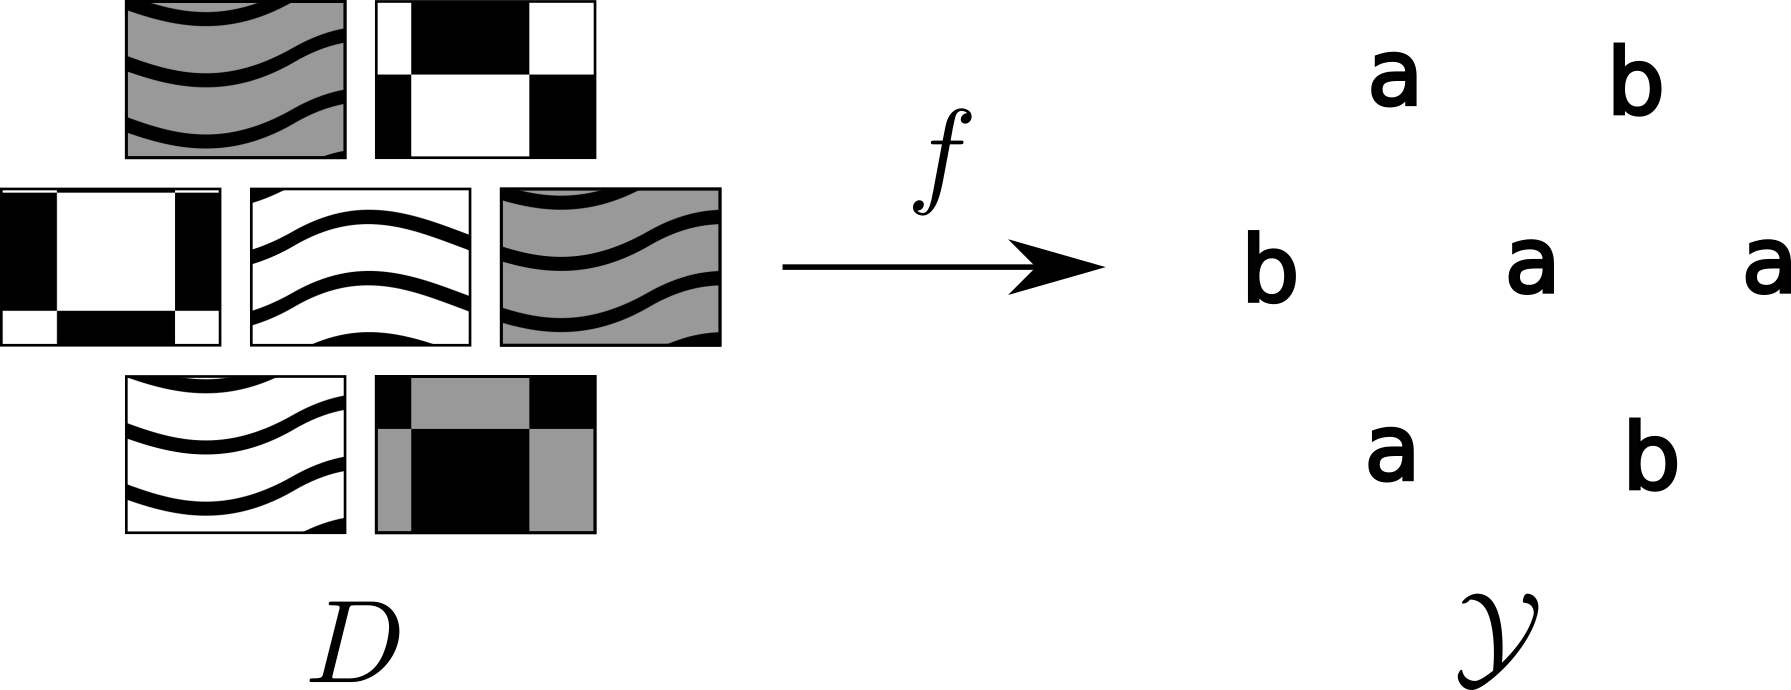
\includegraphics[width=0.6\textwidth]{tl_0}\\
  Initial configuration\\
  \vspace{2em}
  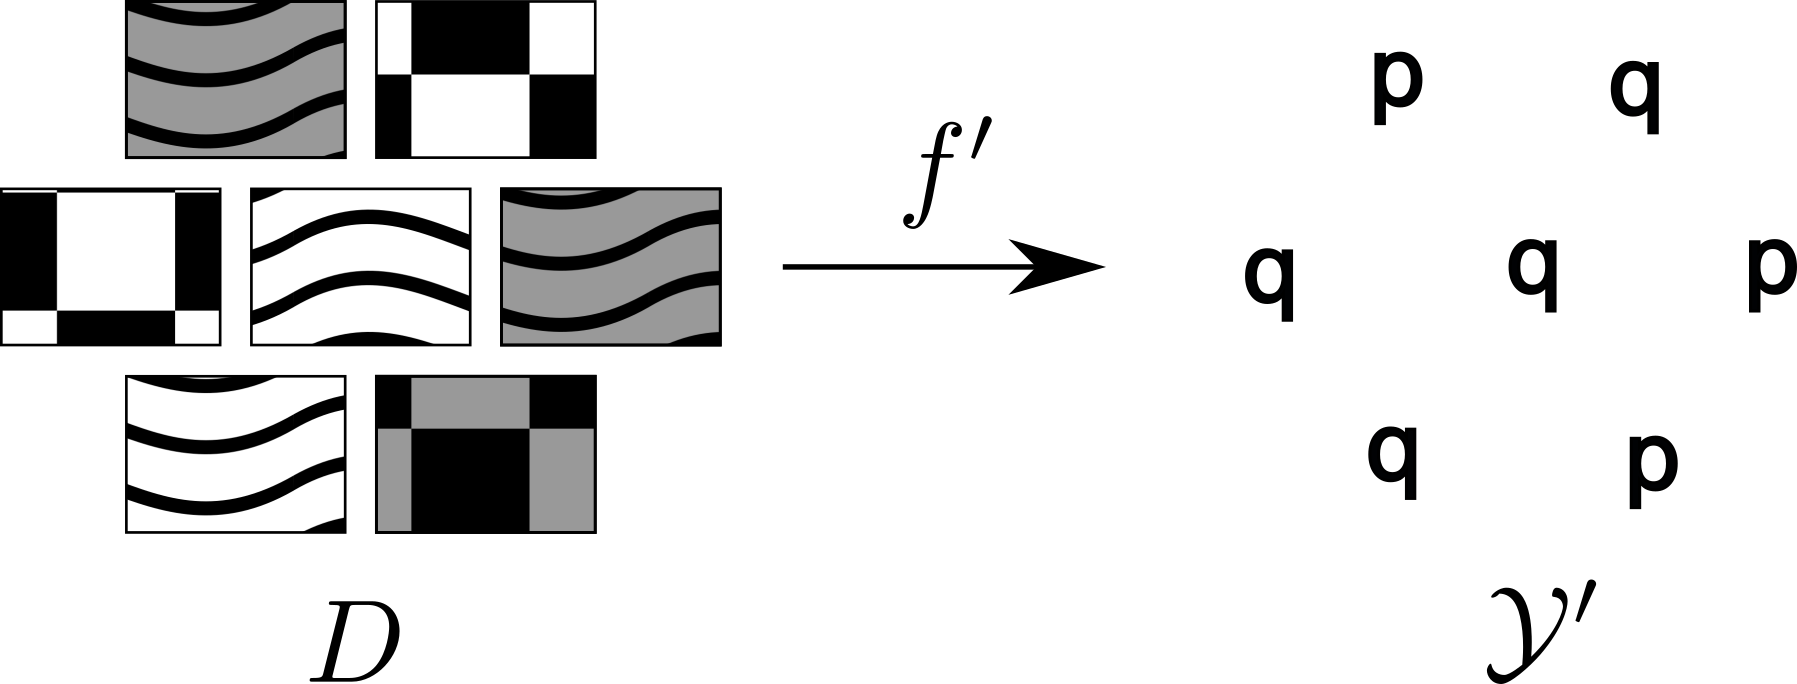
\includegraphics[width=0.6\textwidth]{tl_inductive}\\
  Inductive transfer learning
\end{figure}


\end{frame}


%%%%%%%%%%%%%%%%%%%%%%%%%%%%%%%%%%%%
\begin{frame}{Types of transfer learning: transductive}

\begin{figure}[ht]
  \centering
  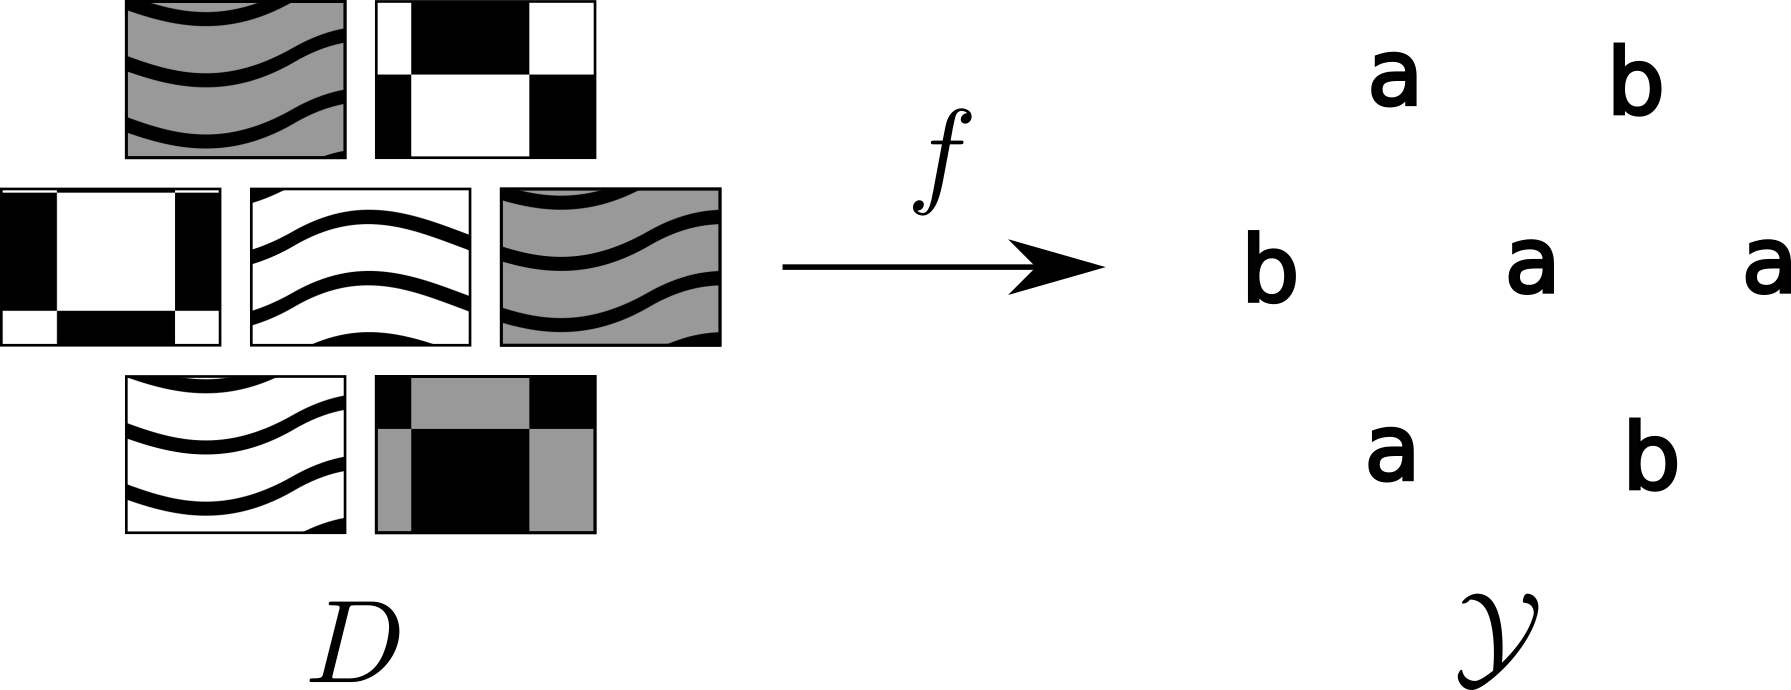
\includegraphics[width=0.6\textwidth]{tl_0}\\
  Initial configuration\\
  \vspace{2em}
  \includegraphics[width=0.6\textwidth]{tl_transductive}\\
  Transductive transfer learning
\end{figure}

\end{frame}


%%%%%%%%%%%%%%%%%%%%%%%%%%%%%%%%%%%%
\begin{frame}{Types of transfer learning: transductive homogeneous}

\begin{figure}[ht]
  \centering
  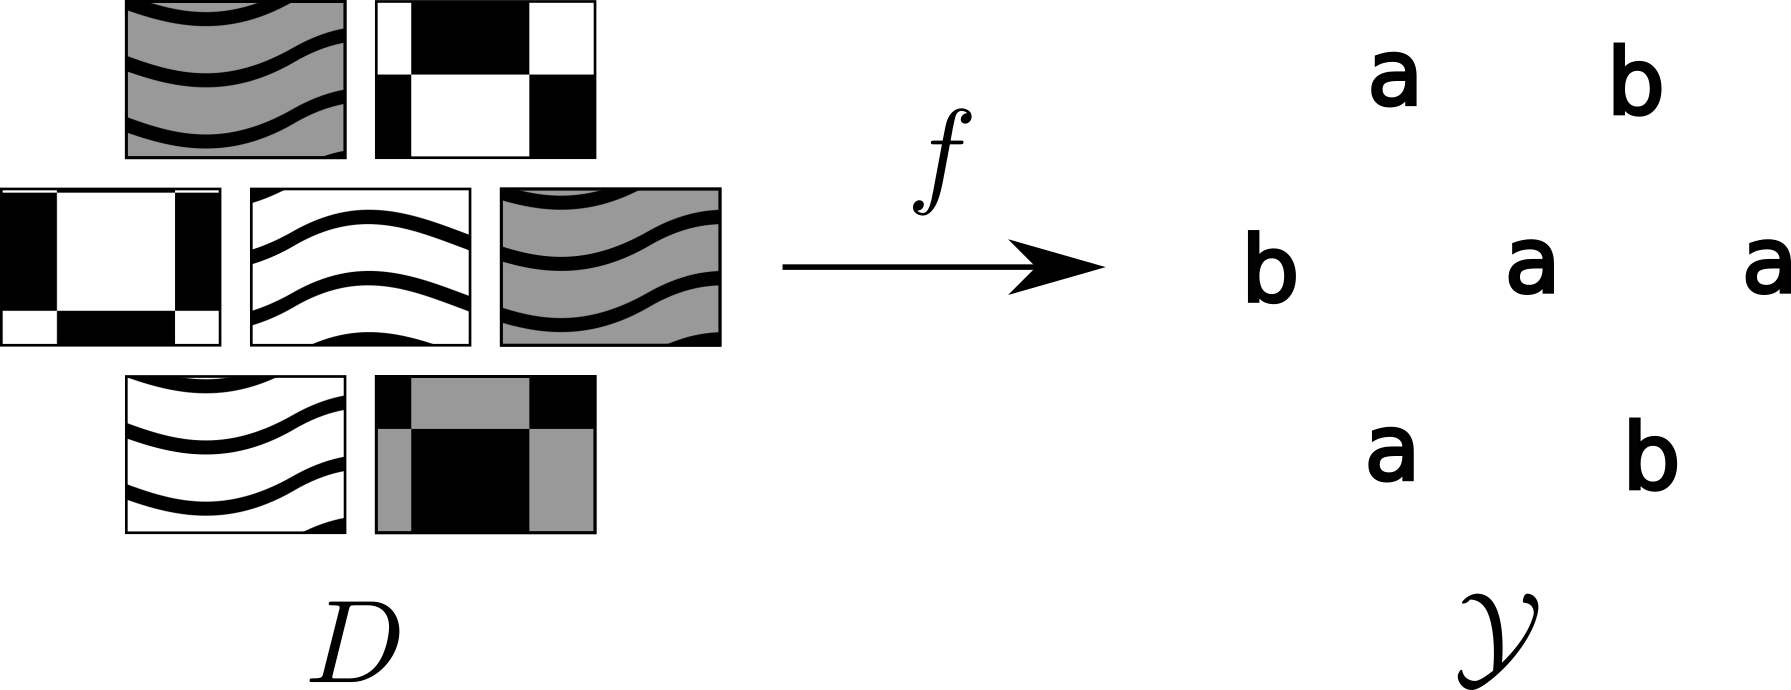
\includegraphics[width=0.6\textwidth]{tl_0}\\
  Initial configuration\\
  \vspace{2em}
  \includegraphics[width=0.6\textwidth]{tl_transductive_homo}\\
  Transductive homogeneous transfer learning
\end{figure}


\end{frame}

%%%%%%%%%%%%%%%%%%%%%%%%%%%%%%%%%%%%
\begin{frame}{Types of transfer learning: transductive heterogeneous}

\begin{figure}[ht]
  \centering
  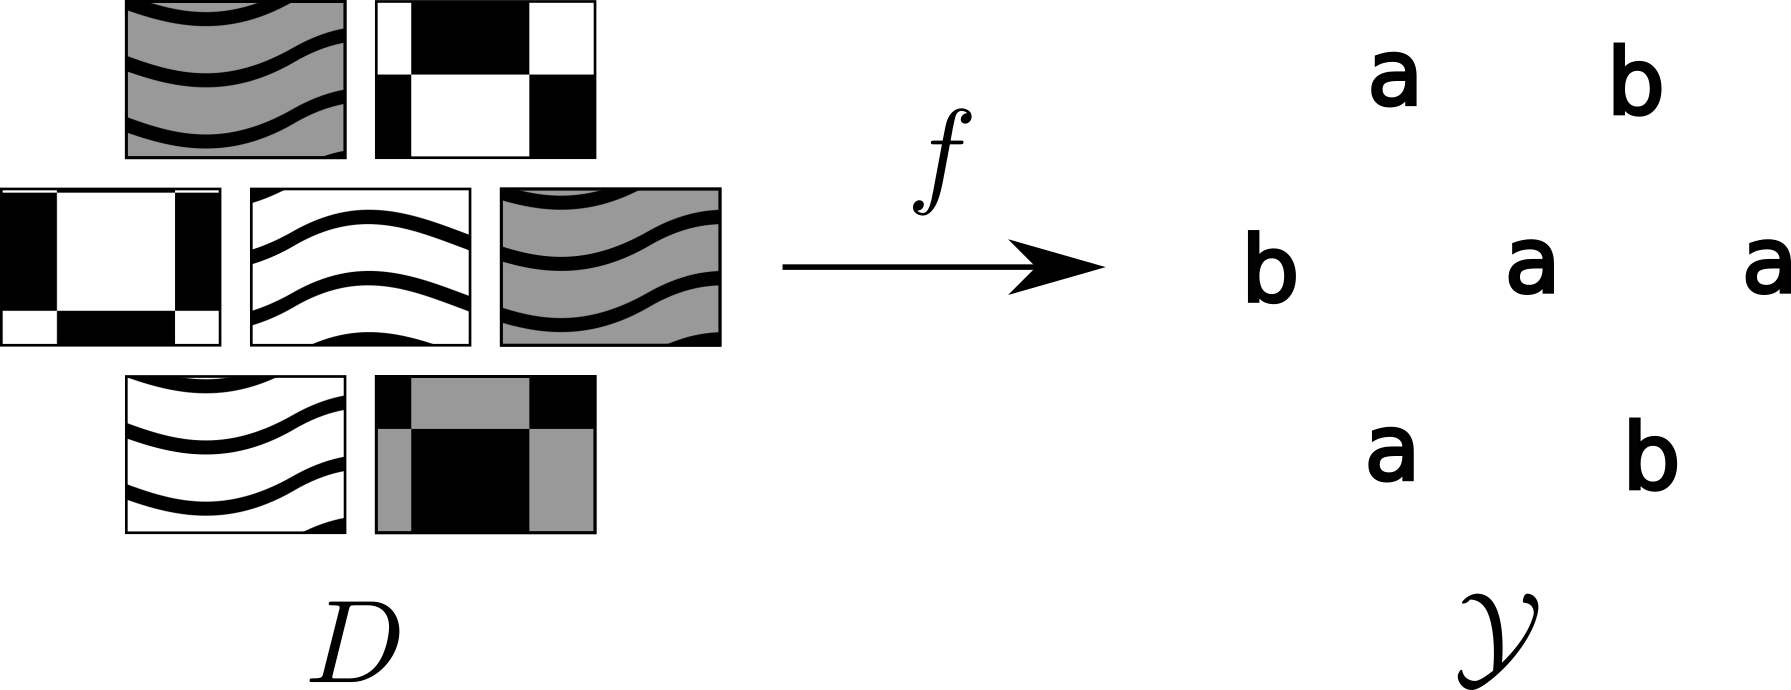
\includegraphics[width=0.6\textwidth]{tl_0}\\
  Initial configuration\\
  \vspace{2em}
  \includegraphics[width=0.6\textwidth]{tl_transductive_hete}\\
  Transductive heterogeneous transfer learning
\end{figure}

\end{frame}

%%%%%%%%%%%%%%%%%%%%%%%%%%%%%%%%%%%%
\begin{frame}{Transfer learning through fine-tuning}

\begin{block}{}
  Suppose that thanks to a training set $(X_0, \mathcal{Y}_0)$ a model $f_{\theta_0}$ has been learnt.

  Transfer learning through fine-tuning consists in learning another model $f_{\theta}$ from a training set $(X, \mathcal{Y})$ using as starting point $f_{\theta_0}$.

  For transfer learning to work, both training sets have to be somehow related and compatible.
\end{block}

\end{frame}

%%%%%%%%%%%%%%%%%%%%%%%%%%%%%%%%%%%%
\begin{frame}{General procedure}

  \begin{itemize}
  \item Choose and existing model, optimized on a data base such as ImageNet. It should be able to process the new data
  \item Remove the last layers of the model and replace them with layers adapted to the task at hand
  \item Fine-tune the resulting model

    \begin{itemize}
    \item Note that some pre-trained layers are often \emph{frozen}
    \end{itemize}
  \end{itemize}

\end{frame}

%%%%%%%%%%%%%%%%%%%%%%%%%%%%%%%%%%%%
\begin{frame}{A reference paper \cite{yosinski_how_2014}}

\begin{block}{}
  Jason Yosinski, Jeff Clune, Yoshua Bengio, Hod Lipson. \textbf{How transferable are features in deep neural networks?} Neural Information Processing Systems, 2014.
\end{block}

The authors devised experiments on the ImageNet database in order to evaluate different fine-tuning strategies and improve our of understanding of these methods.

\end{frame}

%%%%%%%%%%%%%%%%%%%%%%%%%%%%%%%%%%%%
\begin{frame}{Experiments configuration}

  \begin{figure}[ht]
    \centering
    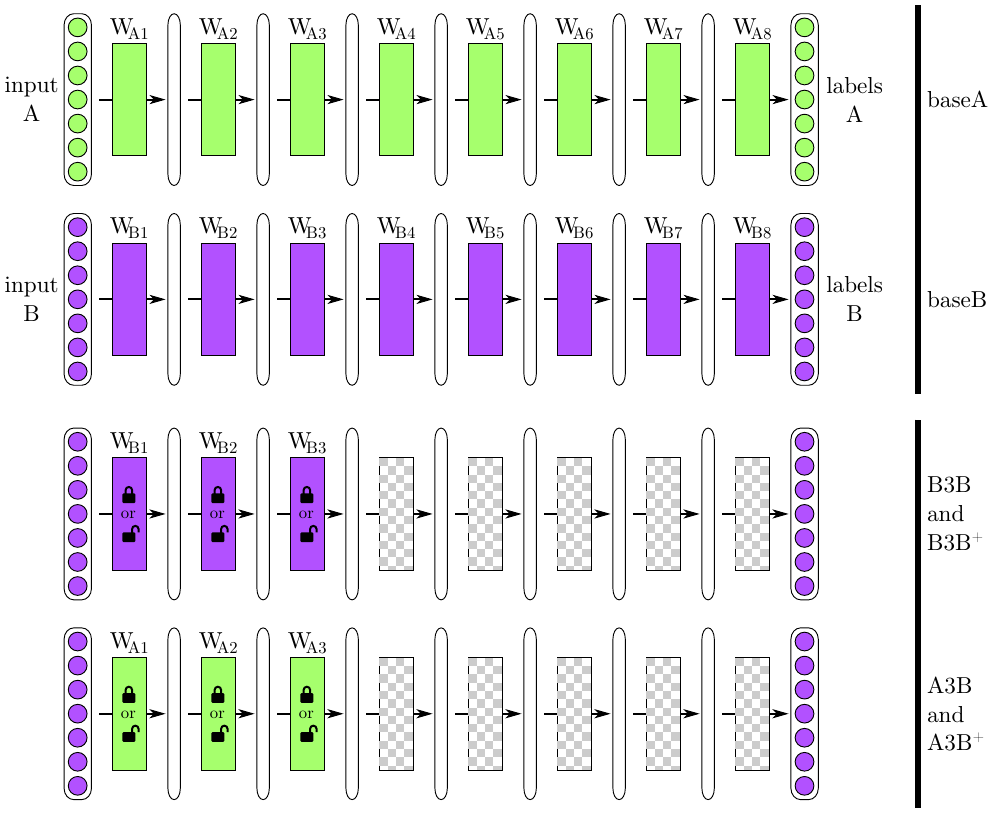
\includegraphics[width=0.8\textwidth]{transfer_learning_exp}\\
    \scriptsize{Layer $n$ at which the network is chopped and retrained}
  \end{figure}

\end{frame}


%%%%%%%%%%%%%%%%%%%%%%%%%%%%%%%%%%%%
\begin{frame}{First experiment configuration}

  \begin{block}{ImageNet data set split}
    \begin{itemize}
    \item Set A: 500 randomly selected classes
    \item Set B: 500 other classes
    \end{itemize}
  \end{block}

\end{frame}


%%%%%%%%%%%%%%%%%%%%%%%%%%%%%%%%%%%%
\begin{frame}{First experiment results}

  \begin{figure}[ht]
    \centering
    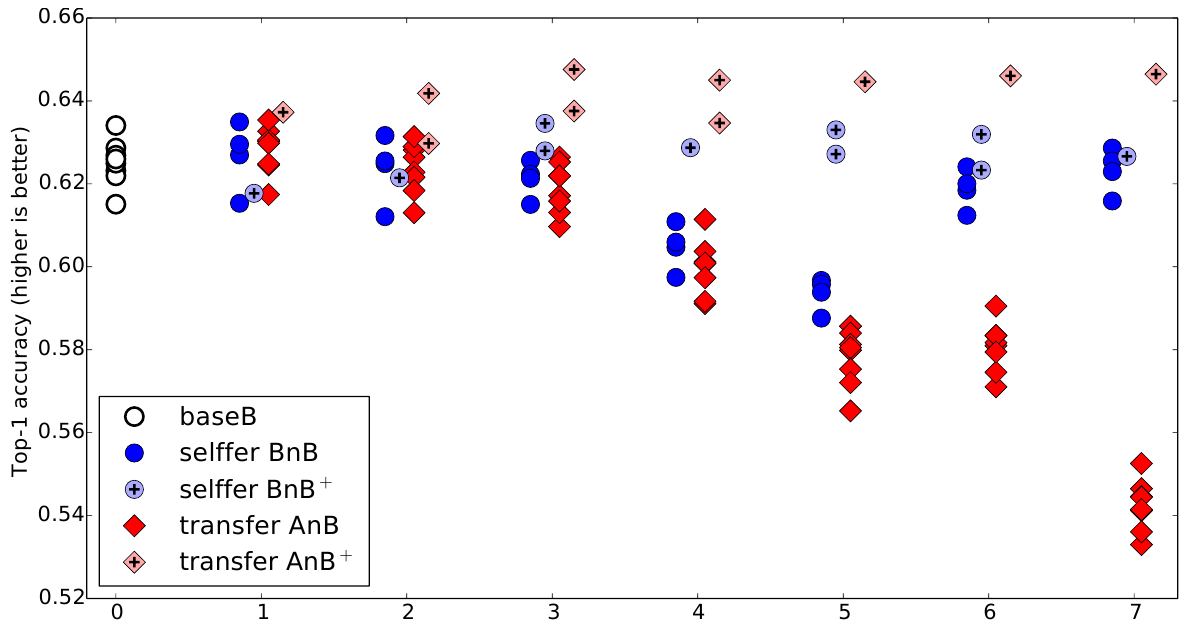
\includegraphics[width=\textwidth]{transfer_learning_res_1}\\
    \scriptsize{Layer $n$ at which the network is chopped and retrained}
  \end{figure}

\end{frame}


%%%%%%%%%%%%%%%%%%%%%%%%%%%%%%%%%%%%
\begin{frame}{First experiment results}

  \begin{figure}[ht]
    \centering
    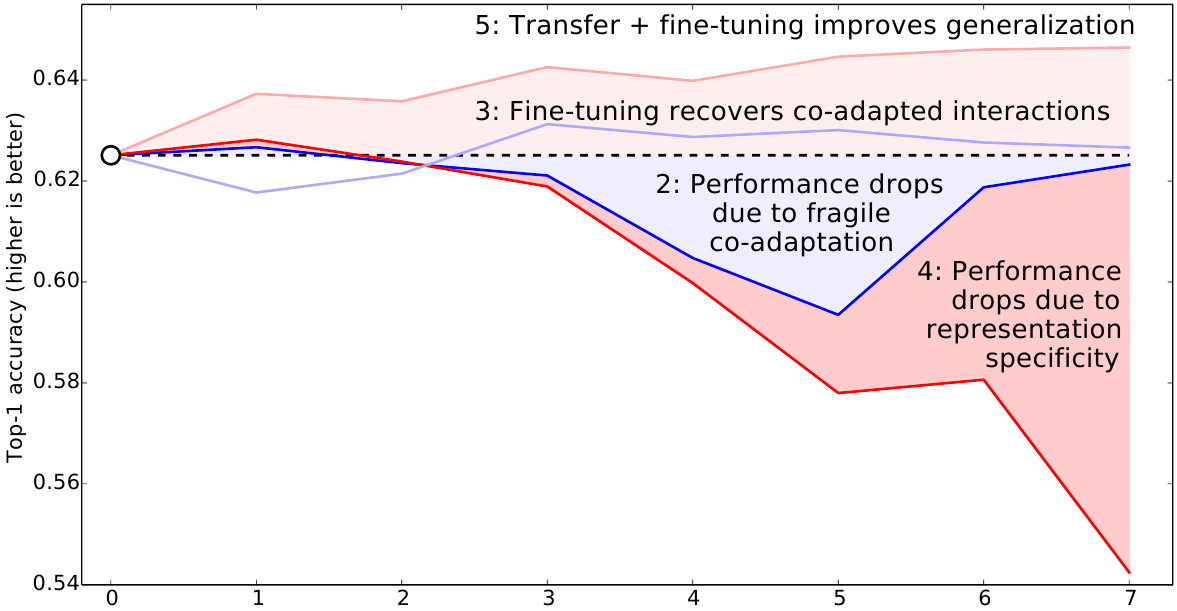
\includegraphics[width=\textwidth]{transfer_learning_res_2}\\
    \scriptsize{Layer $n$ at which the network is chopped and retrained}
  \end{figure}


\end{frame}

%%%%%%%%%%%%%%%%%%%%%%%%%%%%%%%%%%%%
\begin{frame}{Second experiment configuration}

  \begin{block}{ImageNet data set split}
    \begin{itemize}
    \item Set A: Man-made objects (551 classes)
    \item Set B: Natural entities (449 classes)
    \end{itemize}
  \end{block}

\end{frame}


%%%%%%%%%%%%%%%%%%%%%%%%%%%%%%%%%%%%
\begin{frame}{Second experiment results}

  \begin{figure}[ht]
    \centering
    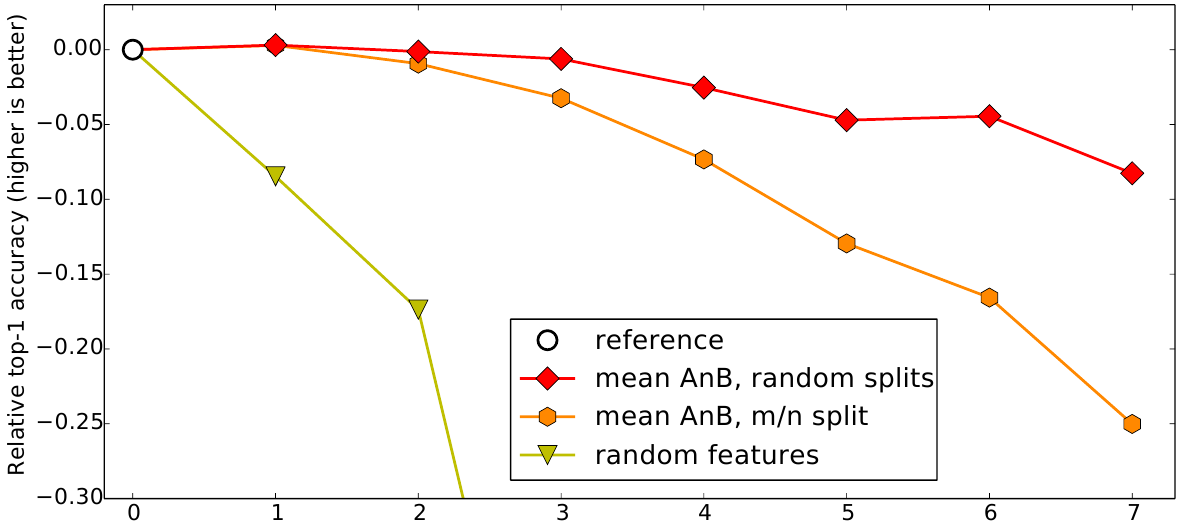
\includegraphics[width=\textwidth]{transfer_learning_res_3}
    \scriptsize{Layer $n$ at which the network is chopped and retrained}
  \end{figure}

\end{frame}



%%%%%%%%%%%%%%%%%%%%%%%%%%%%%%%%%%%%
\begin{frame}{Experiments conclusions}

\begin{itemize}
\item Two separate issues with transfer learning:
  \begin{itemize}
  \item Specificity of high level features
  \item Co-adaptation of neurons on neighboring layers
  \end{itemize}
\item Transfer learning is less efficient when the sets are more dissimilar (at least when the pre-trained weights are frozen)
\item Generalization performance can be boosted by transfer learning
\end{itemize}

\end{frame}


%%%%%%%%%%%%%%%%%%%%%%%%%%%%%%%%%%%%
%% \begin{frame}{Example: Deep learning for galaxy surface brightness profile fitting \cite{tuccillo_deep_2018} }

%% \begin{block}{Task}
%%   To estimate brightness profile parameters (magnitude, half light radius, Sérsic index and axis ratio) of early galaxy images.

%% \end{block}

%%   Data: Cosmic Assembly Near-infrared Deep Extragalactic Legacy Survey (CANDELS), Hubble Space Telescope (HST)

%% \end{frame}

%% %%%%%%%%%%%%%%%%%%%%%%%%%%%%%%%%%%%%
%% \begin{frame}{Hubble space telescope}

%% \begin{figure}[ht]
%%   \centering
%%   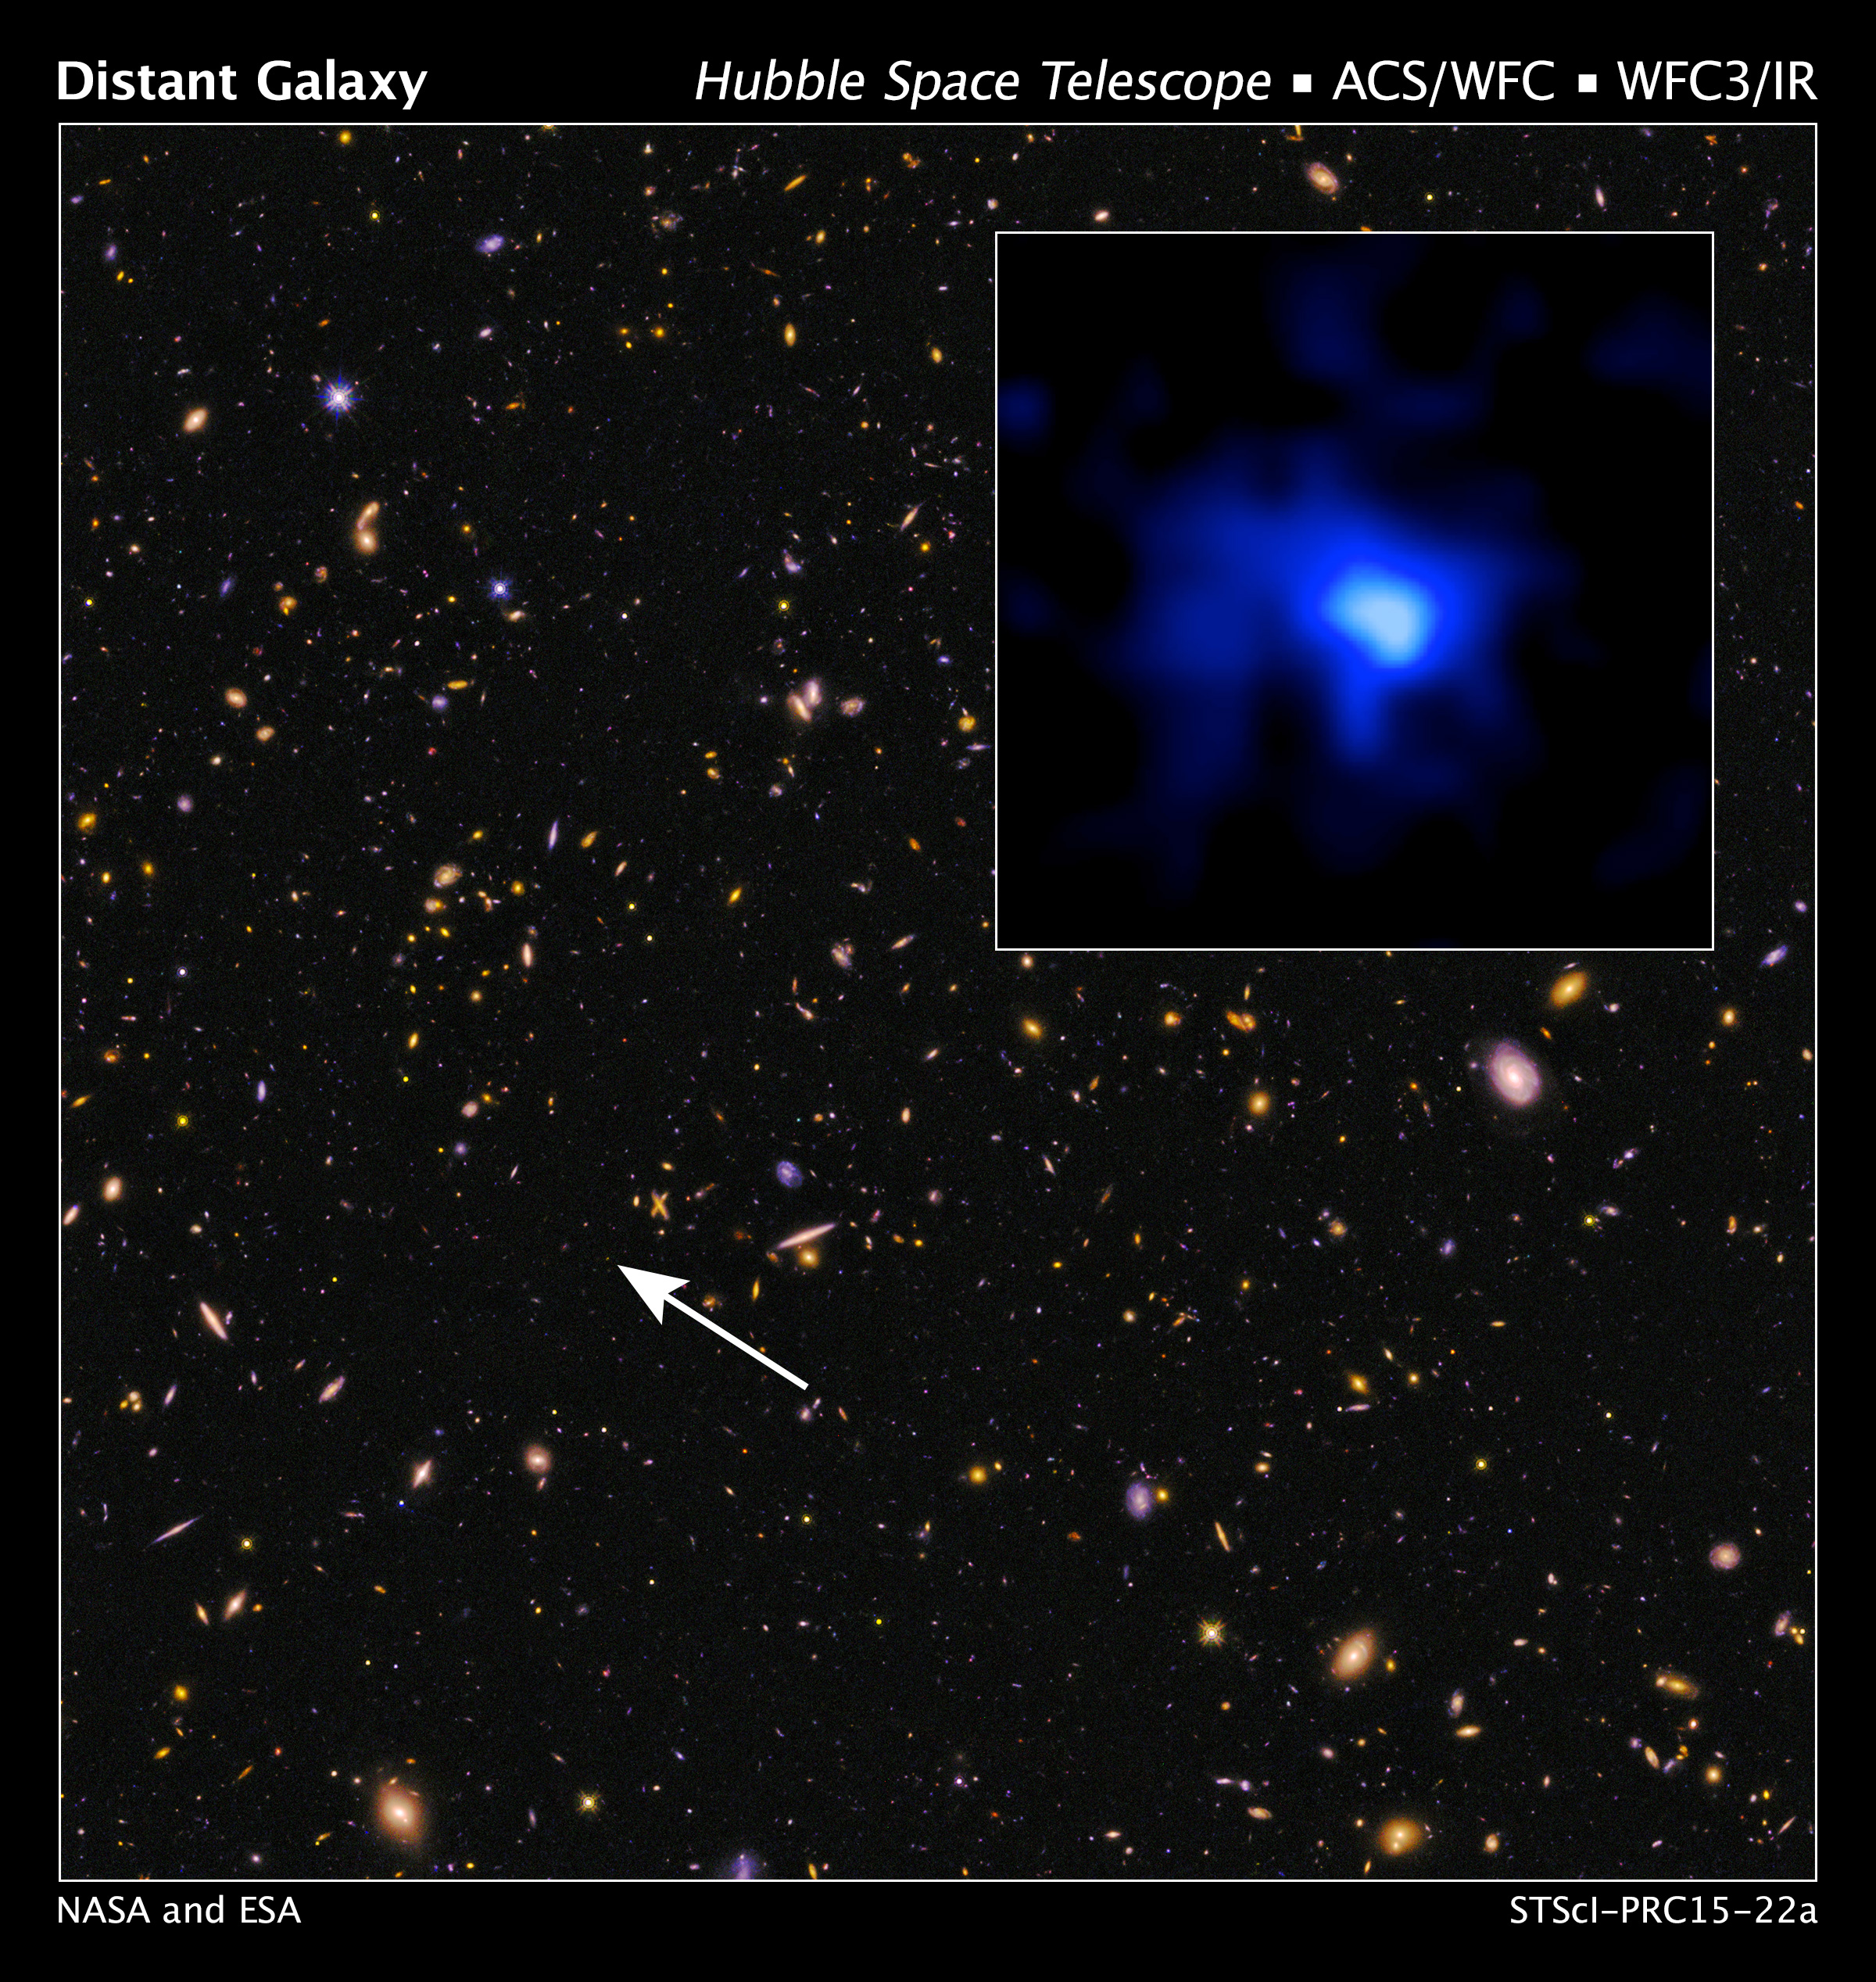
\includegraphics[width=0.5\textwidth]{HST_galaxy.jpg}
%% \end{figure}

%% The farther away the galaxies, the younger they are. These young galaxies bring precious information to improve our understanding of the formation of our universe.

%% \end{frame}


%% %%%%%%%%%%%%%%%%%%%%%%%%%%%%%%%%%%%%
%% \begin{frame}{CANDELS \cite{grogin_candels_2011}}

%% \begin{figure}[ht]
%%   \centering
%%   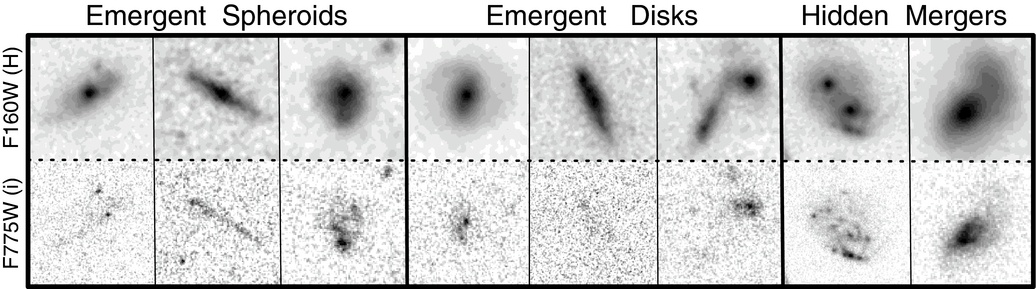
\includegraphics[width=\textwidth]{candels.jpg}
%% \end{figure}

%% Only modality F160W was used in \cite{tuccillo_deep_2018}.

%% \end{frame}


%% %%%%%%%%%%%%%%%%%%%%%%%%%%%%%%%%%%%%
%% \begin{frame}{Available data}

%% Obtaining measures from the real images is done in practice with GALFIT, but the procedure is not totally automatic.

%% \begin{itemize}
%% \item Real annotated data: 5000 images from the van der Wel et al. (2012) catalog
%% \item Simulated data
%% \end{itemize}

%% \end{frame}


%% %%%%%%%%%%%%%%%%%%%%%%%%%%%%%%%%%%%%
%% \begin{frame}{Adopted strategy}

%% \begin{itemize}
%% \item Learning using $55\,000$ simulated images, with corresponding measures
%% \item First test on simulated data and comparison with GALFIT
%% \item Transfer learning using $4\,000$ images from the van der Wel catalog
%% \item Test on real data using the $1\,000$ remaining images
%% \end{itemize}

%% \end{frame}

%% %%%%%%%%%%%%%%%%%%%%%%%%%%%%%%%%%%%%
%% \begin{frame}{Results on simulated data}

%% \begin{figure}[ht]
%%   \centering
%%   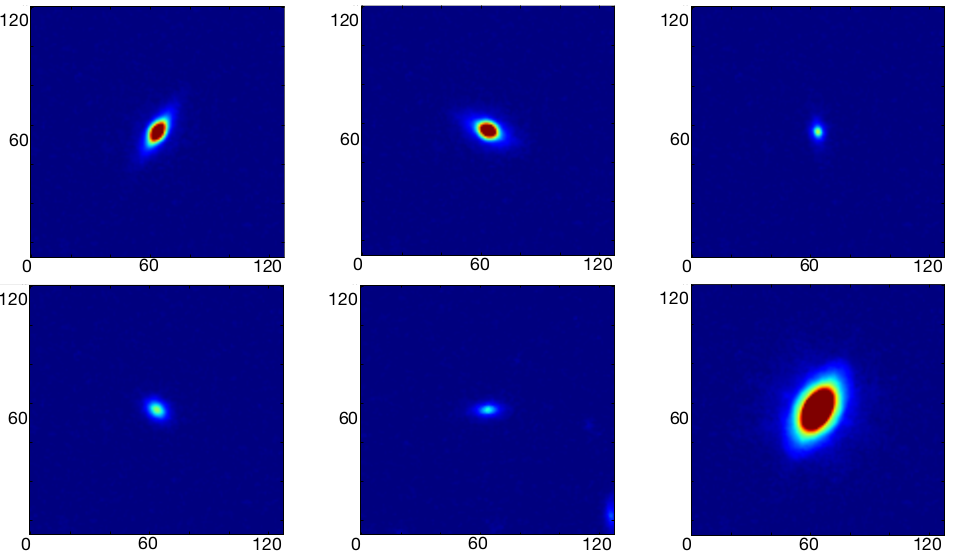
\includegraphics[width=0.5\textwidth]{gal_simu}
%% \end{figure}

%% \begin{columns}
%%   \begin{column}{.5\textwidth}
%% \begin{figure}[ht]
%%   \centering
%%   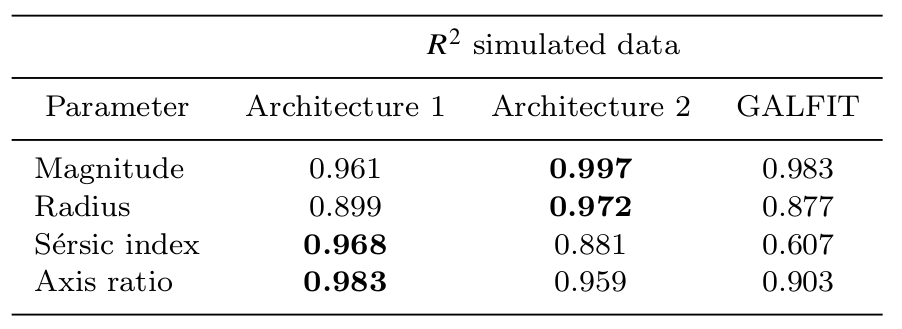
\includegraphics[width=\textwidth]{deeplegato_galfit_sim_res}
%% \end{figure}

%%   \end{column}

%%   \begin{column}{.5\textwidth}
%%     \scriptsize
%% Computing time (5000 galaxies):
%% \begin{itemize}
%% \item GALFIT (CPU): 12600 s
%% \item NN (CPU): 200 s
%% \item NN (GPU): 4 s
%% \end{itemize}

%%   \end{column}
%% \end{columns}

%% \end{frame}

%% %%%%%%%%%%%%%%%%%%%%%%%%%%%%%%%%%%%%
%% \begin{frame}{Results on real data: examples}

%% \begin{columns}
%%   \begin{column}{.5\textwidth}
%% \begin{figure}[ht]
%%   \centering
%%   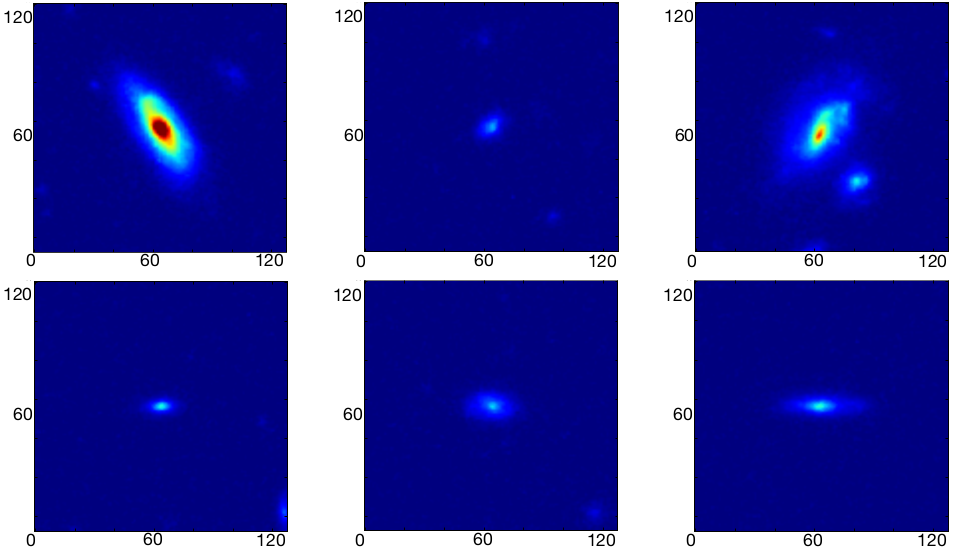
\includegraphics[width=\textwidth]{gal_real_ok}\\
%%   \scriptsize{Correct results}
%% \end{figure}

%%   \end{column}

%%   \begin{column}{.5\textwidth}
%% \begin{figure}[ht]
%%   \centering
%%   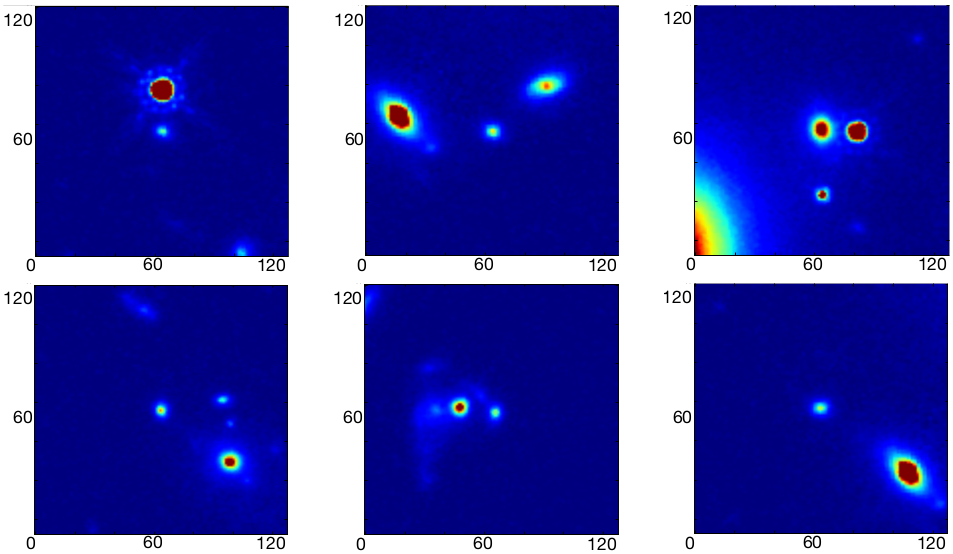
\includegraphics[width=\textwidth]{gal_real_notok}\\
%%   \scriptsize{Incorrect results}
%% \end{figure}

%%   \end{column}
%% \end{columns}

%% \end{frame}



%% %%%%%%%%%%%%%%%%%%%%%%%%%%%%%%%%%%%%
%% \begin{frame}{Results on real data}

%% \begin{figure}[ht]
%%   \centering
%%   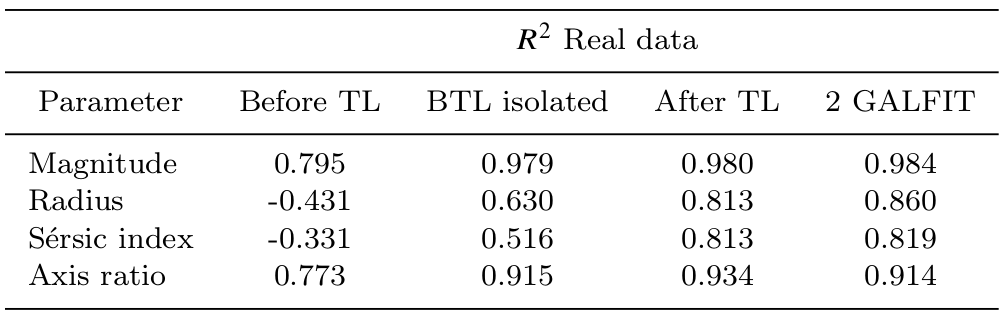
\includegraphics[width=0.75\textwidth]{deeplegato_galfit_real_res}
%% \end{figure}

%% 2 GALFIT: comparison between two sets of measures obtained with GALFIT, the first as given in the van der Wel et al. (2012) catalog, and the second obtained by Dimauro et al. (2017).

%% \end{frame}



%%%%%%%%%%%%%%%%%%%%%%%%%%%%%%%%%%%%%%%%%%%%%%%%%%
\section*{Conclusion}

%%%%%%%%%%%%%%%%%%%%%%%%%%%%%%%%%%%%
\begin{frame}{Conclusion}

  \begin{block}{}
    \begin{itemize}
    \item You now know the basics to tackle many computer vision problems with deep learning.
    \item But there are many other topics of interest:
      \begin{itemize}
      \item Non supervised methods, including autoencoders and generative adversarial networks (next lectures)
      \item Self-supervision, low supervision
      \item Recurrent networks
      \item Anomaly detection
      \item Attention mechanisms
      \item etc.
      \end{itemize}
    \end{itemize}
  \end{block}

\end{frame}



%%%%%%%%%%%%%%%%%%%%%%%%%%%%%%%%%%%%%%%%%%%%%%%%%%
\section*{References}

%%%%%%%%%%%%%%%%%%%%%%%%%%%%%%%%%%%%%%%%%%%%%%%%%%

\frame[allowframebreaks]{

  \scriptsize

  \frametitle{References}

  %\bibliographystyle{amsalpha}
  %\bibliographystyle{apalike}

  \bibliography{../../edf.bib}

  \normalsize

}




\end{document}
